%--------------------------------------------------------------------
% Эта преамбула с комментариями для написания лабораторных работ по
% физике. В еe основе информация из книги С. М. Львовского "Набор и
% верстка в пакете Latex", а также материалы по курсу "Документы и
% презентации в Latex" от ВШЭ https://www.coursera.org/learn/latex. Ну
% и мой опыт (1 год и 16 лабораторных работ + 2 Вопроса по выбору)
% Автор - Баринов Леонид
% Дата - 06.08.2019
%--------------------------------------------------------------------
%--------------------------------------------------------------------
% Для начала необходимо определиться с типом документа. Оптимальный
% (на мой взгляд) вариант - article. Также существуют типы book,
% report, proc и другие. Также в необязательном аргументе можно
% указать тип страницы и размер шрифта. Стандарт по умолчанию - А4 и
% 12 (иногда 10) шрифт. Необязательный аргумент шрифта может принимать
% только 3 параметра - 10, 11, 12 (pt).

\documentclass[a4paper, 12pt]{article}

%--------------------------------------------------------------------
% Чтобы использовать другие размеры шрифта используется пакет
% extsizes. Он позволяет указывать в \documentclass такие размеры - 8,
% 9, 10, 11, 12, 14, 17, 20 (pt). При указании других размеров могут
% возникать различные проблемы.

\usepackage{extsizes}

%--------------------------------------------------------------------
% Необходимо определиться с кодировкой документа. Идеального варианта
% для русского языка не существует - каждый чем-то немного плох. Для
% особо интересующихся - Приложение И в 5 издании книги Львовского. Я
% воспользовался вариантом, предлагаемым на курсе по Latex от ВШЭ.

\usepackage[T2A]{fontenc}
\usepackage[utf8]{inputenc}

%--------------------------------------------------------------------
% Для соблюдения типографских традиций (оказывается такие существуют)
% различных стран создан пакет babel. Самое заметное его действие -
% latex научиться переносить слова того языка, который вы укажите.
% Можно указать несколько языков через запятую. Основной язык
% документа указывается последним.

\usepackage[english,russian]{babel}

%--------------------------------------------------------------------
% Перейдем к заданию полей документа. Есть несколько способов, но
% самый простой из них - это воспользоваться пакетом geometry, который
% позволяет определить все поля документа (начиная с краев листа, что
% важно, так как некоторые другие способы позволяют это сделать только
% косвенно)

\usepackage{geometry}
\geometry{top=25mm}
\geometry{bottom=35mm}
\geometry{left=35mm}
\geometry{right=20mm}

%--------------------------------------------------------------------
% От полей логично перейти к колонтитулам. Тут нам поможет пакет
% fancyhdr. Для него существует 6 колонтитулов - верхний, левый;
% верхний, по центру; верхний, правый и такие же нижние. По умолчанию
% номер страницы находится снизу по центру, а также существует
% линейка, очерчивающие верхний колонтитул. Мне показалось интересным
% сделать колонтитулы схожие с колонтитулами в лабнике. 

\usepackage{fancyhdr}
\pagestyle{fancy}
\renewcommand{\sectionmark}[1]{\markboth{#1}{}} 
% \renewcommand{\headrulewidth}{0mm} % Если необходимо убрать линейку,
% или изменить ее длину
% \lfoot{} % Нижний левый
% \rfoot{} % Нижний правый
% \rhead{} % Верхний правый
% \chead{} % Верхний в центре
\lhead{\thepage} % Номер страницы в левом верхнем углу
\cfoot{} % Оставить нижний колонтитул без цифры

%--------------------------------------------------------------------
% Самое время научиться работать с формулами. А точнее добавить пакеты
% от Американского математического общества, которые позволять
% пользоваться большим количеством математических символов.

\usepackage{amsmath,amsfonts,amssymb,amsthm,mathtools}

%--------------------------------------------------------------------
% Также очень хочется пользоваться русскими буквами в формулах, для
% этого подключаем пакет mathtext, который добавляет окружение
% \text{}. Внутри него можно писать русские буквы в математическом
% режиме.

\usepackage{mathtext}

%--------------------------------------------------------------------
% Большим преимуществом вашего pdf документа будет возможность поиска
% в нем по словам или буквами. (Например, в Ивановнике это
% невозможно)

\usepackage{cmap}

%--------------------------------------------------------------------
% Куда же в физике без картинок и графиков? Давайте исправим
% эту недоработку

\usepackage{graphicx}
\graphicspath{images/} % Необходимо, если рисунки
% находятся в другой папке

%--------------------------------------------------------------------
% graphicx не позволяет вставлять обтекаемые рисунки, но на
% практике они очень нужны. Для этого существует пакет wrapfig

\usepackage{wrapfig}

%--------------------------------------------------------------------
% latex вставляет рисунки по определенному алгоритму. Его,
% конечно, можно менять, но это не настолько просто. Как
% правило, хочется, чтобы картинка располагалась там, где мы это
% указали в коде. Для этого существует несколько пакетов, один из
% них floatrow. Он позволяет для окружения figure указывать
% необязательный аргумент - H (именно большое h), что на latex'овском
% языке означает: вставить картинку здесь и только здесь. (даже если
% облик документа несколько пострадает)

\usepackage{floatrow}

%--------------------------------------------------------------------
% По правилам оформления рисунок всегда должен быть подписан. Для
% этого существует команда \caption{}. Но обычные настройки caption
% меня не совсем устроили. Хотелось сделать подпись меньше
% основного шрифта, а также слово Рис жирным и использовать
% разделитель точку, а не двоеточие. В этом помогает пакет,
% который называется caption (совпадение?)

\usepackage[margin=10pt,font=small,labelfont=bf,labelsep=period]{caption}

%--------------------------------------------------------------------
% Последним важным пунктом остались таблицы. Ведь куда-то нужно
% заносить результаты измерений. На данный момент во время выполнения
% лабораторных работ я заношу результаты в таблицу excel, а потом с
% помощью сайта www.tablesgenerator.com превращаю в таблицу latex и
% дооформляю.

\usepackage{array,tabularx,tabulary,booktabs}

%--------------------------------------------------------------------
% После excel есть ощущения, что везде объединить колонки или строки
% легко. В latex не совсем так. Помогают пакеты multirow, multicol. 

\usepackage{multirow}
\usepackage{multicol}

%--------------------------------------------------------------------
% Иногда могут потребоваться длинные таблицы на несколько страниц.
% Обычные таблицы latex воспринимает как одну букву. И
% становиться понятно, почему возникают проблемы при переносе
% обычной таблицы. (Ведь нельзя же перенести одну букву!). Поэтому
% вместо обычной таблицы нужна длинная таблица.

\usepackage{longtable}

%--------------------------------------------------------------------
% Часто в таблице хочется сделать перенос текста или формулы. Просто
% так это сделать не получиться из-за синтаксиса tabular. Для этого
% каждый раз необходимо создавать новое окружение tabular, что
% утомительно. Поэтому можно ввести команду \specialcell
% (назвать можно по-любому)
    
\newcommand{\specialcell}[2][c]{%
	\begin{tabular}[#1]{@{}c{}}#2\end{tabular}}

%--------------------------------------------------------------------
% Когда в таблице много колонок и строк, кажется, что они находятся
% слишком близко к друг другу. Можно переопределить
% несколько параметров, чтобы выглядело лучше. Это можно сделать либо
% в преамбуле, либо непосредственно в документе. Первое
% переопределение отвечает за интервал между строками, второе за
% интервал между колонками

% \renewcommand{\arraystretch}{1.8} 
% \renewcommand{\tabcolsep}{1cm} 

%--------------------------------------------------------------------
% В русской типографской традиции принято начинать каждый новый абзац
% с красной строки. Даже первый после заголовка (или подзаголовка).
% Чтобы каждый раз не ставить красную строку вручную существует пакет
% indentfirst

\usepackage{indentfirst}

%--------------------------------------------------------------------
% Некоторые модификаторы начертания

\usepackage{soul}
\usepackage{soulutf8}
 
\begin{document}
\thispagestyle{empty}
\begin{center}
    \textit{Федеральное государственное автономное образовательное\\ учреждение высшего образования }

    \vspace{0.5ex}

        \textbf{«Московский физико-технический институт\\ (национальный исследовательский университет)»}
\end{center}

\vspace{10ex}

\begin{center}
    \vspace{13ex}

    \so{\textbf{Лабораторная работа №_._._}}

    \vspace{1ex}

    по курсу общей физики

    на тему:

    \textbf{\textit{<<>>}}

    \vspace{30ex}

    \begin{flushright}
        \noindent
        \textit{Работу выполнил:}\\  
        \textit{Баринов Леонид \\(группа Б02-827)}
    \end{flushright}
    \vfill
    Долгопрудный \\2019
\newpage
\setcounter{page}{1}
\fancyhead[R]{\nouppercase{\leftmark}}	
\end{center}

\section{Аннотация}
В работе будет определено отношение заряда электрона к его массе методом фокусировки и
методом магнетрона.
\section{Теоретические сведения}
На заряд $q$, движущийся со скоростью $\upsilon$ в магнитном поле $B$ действует сила Лоренца:
\[
\vec F = q\vec \upsilon \times\vec B
\] 

Изначальную скорость движения электрона можно найти, зная разность потенциалов $V$, пройденную
электронном:
\[
\frac{m\upsilon^2}{2} = eV
\] 

Электрон движется в магнитном поле под некоторым углом $\alpha$ к вектору магнитной индукции.
Разложим скорость на две составляющие:
\begin{equation*}
    \begin{aligned}
        \upsilon_\bot= \upsilon \sin\alpha, & & \upsilon_\| = \upsilon \cos \alpha
    \end{aligned}
\end{equation*}

Сила $F$ является центростремительной силой, поэтому:
\[
m\frac{\upsilon_\bot^2}{R} = e\upsilon_\bot B
\] 

В направлении поля $B$ на электрон не действуют никакие силы, следовательно в этом направлении
электрон движется равномерно со скоростью $\upsilon_\|$. Траектория электрона представляет
собой винтовую линию. Следовательно, время одного оборота $T_\text{с}$ (циклотронный периода) равно
$T = 2\pi R/\upsilon_\bot$. Выражая $R$ и $\upsilon_\bot$ из предыдущих формул получаем:
\[
    T_\text{с} = \frac{2\pi m}{eB}
\] 

За это время электрон проходит вдоль магнитного поля расстояние
\[
L = \upsilon_\| T_\text{c} = \frac{2\pi \upsilon \cos \alpha}{(e/m) B}
\] 

Когда углы невелики формулу можно записать в виде:
\[
    L \approx \frac{2\pi \upsilon}{(e/m)B}
\] 

Таким образом, расстояние $L$ не зависит от угла $\alpha$ (для малых углов),так что все электроны,
вышедшие из одной точки, после одного оборота вновь соберутся в точке в одной точке
(сфокусируются). Обозначим через $B_\text{ф}$ индукцию магнитного поля, при котором наступает
фокусировка. Исходя из предыдущих формул получим:
\begin{equation}
    \frac{e}{m} = \frac{8\pi^2V}{L^2B_\text{ф}^2}  
\end{equation}

\subsection*{Метод магнитной фокусировки}
В этом методе удельный заряд электрона вычисляется по формуле:
\begin{equation}
    \frac{e}{m} = \frac{8\pi^2 V}{l^2}\left(\frac{n^2}{B_\text{ф}^2}\right)
\end{equation}
где $V$ -- ускоряющий потенциал в электронной трубке, $l$ -- путь электрона, $B_\text{ф}$ --
фокусирующие поле, $n$ -- номер фокуса.

\begin{wrapfigure}{r}{0.33\linewidth}
    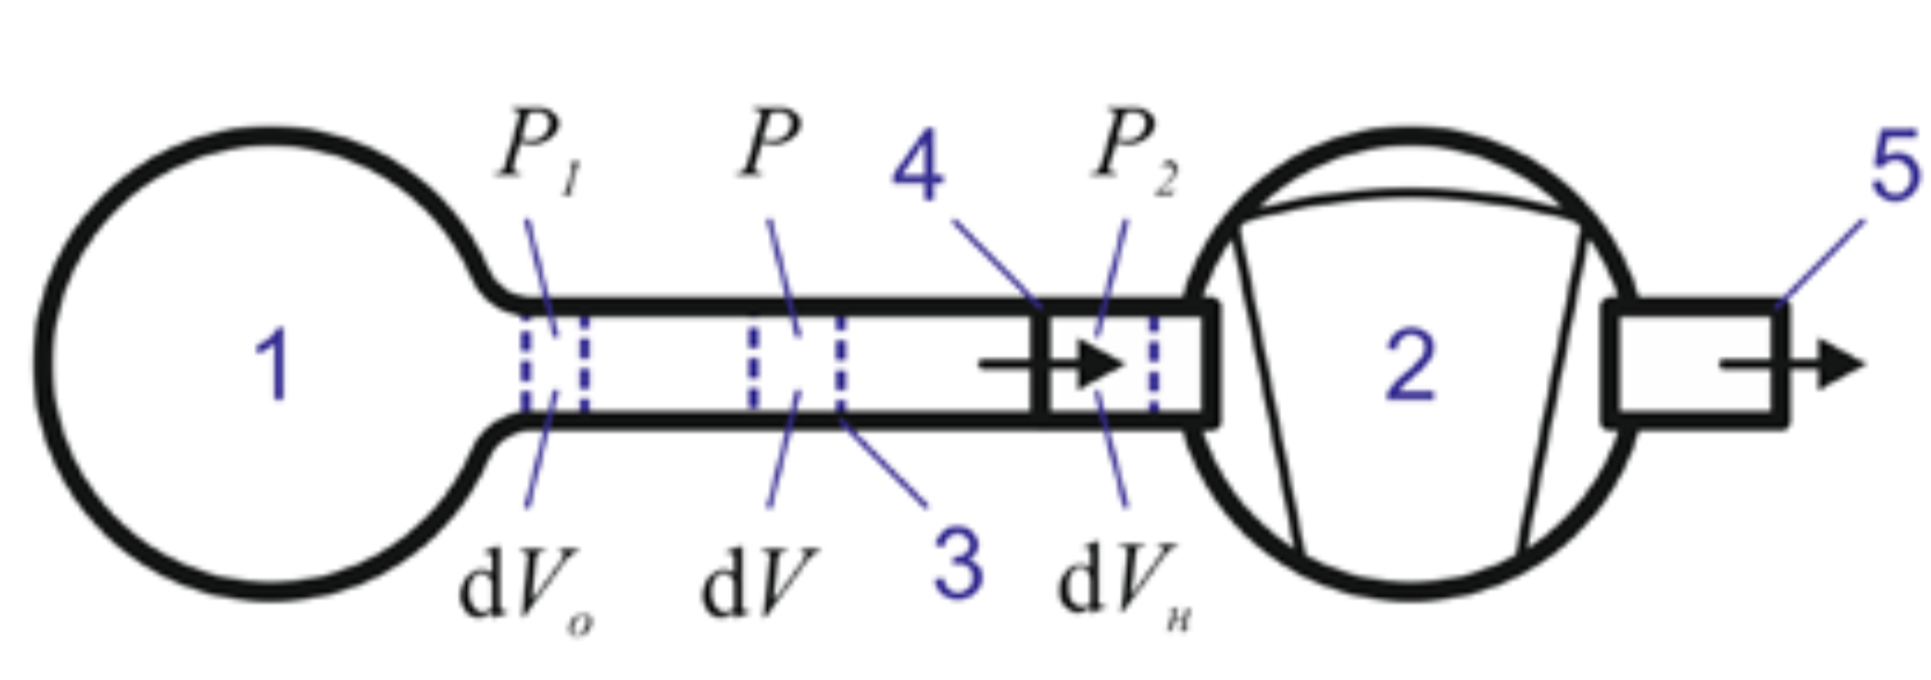
\includegraphics[width=\linewidth]{1}
    \captionsetup{justification=centering}
    \caption{Зависимость анодного тока от индукции магнитного поля в соленоиде}
\end{wrapfigure}
\subsection*{Метод магнетрона}
В этом методе заряд электрона определяется по формуле:
\begin{equation}
    \frac{e}{m} = \frac{8V_\text{а}}{B_\text{кр}^2 r_\text{а}^2}
\end{equation}
где $V_\text{а}$ -- анодное напряжение, $B_\text{кр}$ -- критическое поле (Рис. 1), $r_\text{а}$ --
радиус анода.

\section{Оборудование}
\subsection*{Метод магнитной фокусировки}
\begin{wrapfigure}[21]{l}{0.3\linewidth}
    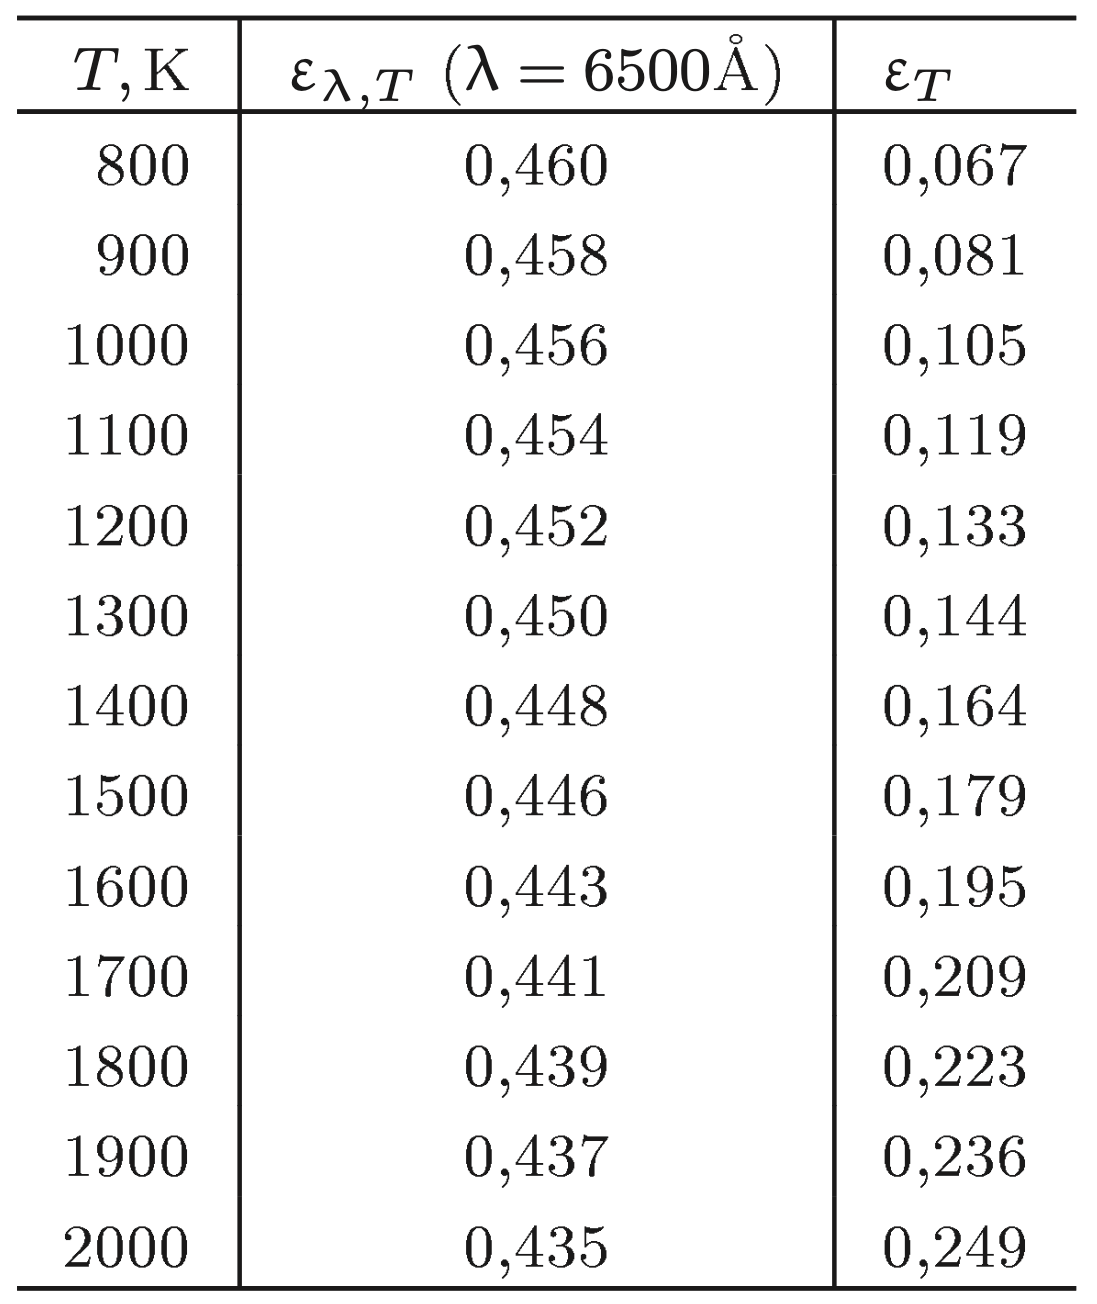
\includegraphics[width=\linewidth]{2}
    \captionsetup{justification=centering}
    \caption{Схема установки для измерений $e/m$ методом магнитной фокусировки}
\end{wrapfigure}
В работе используется: электронно-лучевая трубка и блок питания к ней; источник постоянного тока;
соленоид; электростатический вольтметр; милливеберметр; ключи.

\subsubsection*{Экспериментальная установка}
Основной частью установки является электронный осциллограф С1-1, трубка которого вынута и
установлена в длинном соленоиде, создающим магнитное поле. Напряжение на отклоняющие пластины и
питание подводятся к трубке многожильным кабелем.

Пучок электронов, вылетающих из катода с разными скоростями. Пропустив пучок сквозь две узких диафрагмы, можно выделить электроны с
практически одинаковой продольной скоростью $\upsilon_\|$. Небольшое переменное напряжение, поступающее с
клеммы <<Контрольный сигнал>> осциллографа на отклоняющие пластины, изменяет только поперечную
составляющую скорости. Угол $\alpha$ отклонения пучка от оси трубки, таким образом, зависит от времени, и электроны прочерчивают на экране трубки светящуюся линию. При увеличении магнитного поля линия на
экране сокращается, постепенно стягиваясь в точку, а затем снова удлиняется. Второе прохождение
через фокус происходит в том случае, когда электроны на пути от катода к экрану описывают два витка
спирали, третье — при трёх витках.

Анодное напряжение, определяющее продольную скорость электронов, измеряется электростатическим киловольтметром.

Магнитное поле в соленоиде создаётся постоянным током (Рис. 2), сила которого регулируется ручками
источника питания и измеряется амперметром A источника. Ключ K служит для изменения направления поля в соленоиде.

Величина магнитного поля определяется с помощью милливеберметра ($mWb$ на Рис. 2). Этот прибор
измеряет изменение магнитного потока, пронизывающего измерительную (пробную) катушку, которая
намотана на один каркас с соленоидом.
\subsection*{Метод магнетрона}
В работе используются: электронная лампа е цилиндрическим анодом; соленоид; источники питания лампы и соленоида; вольтметр постоянного тока; миллиамперметр, амперметр.
\subsubsection*{Экспериментальная установка}

\begin{wrapfigure}{r}{0.5\linewidth}
    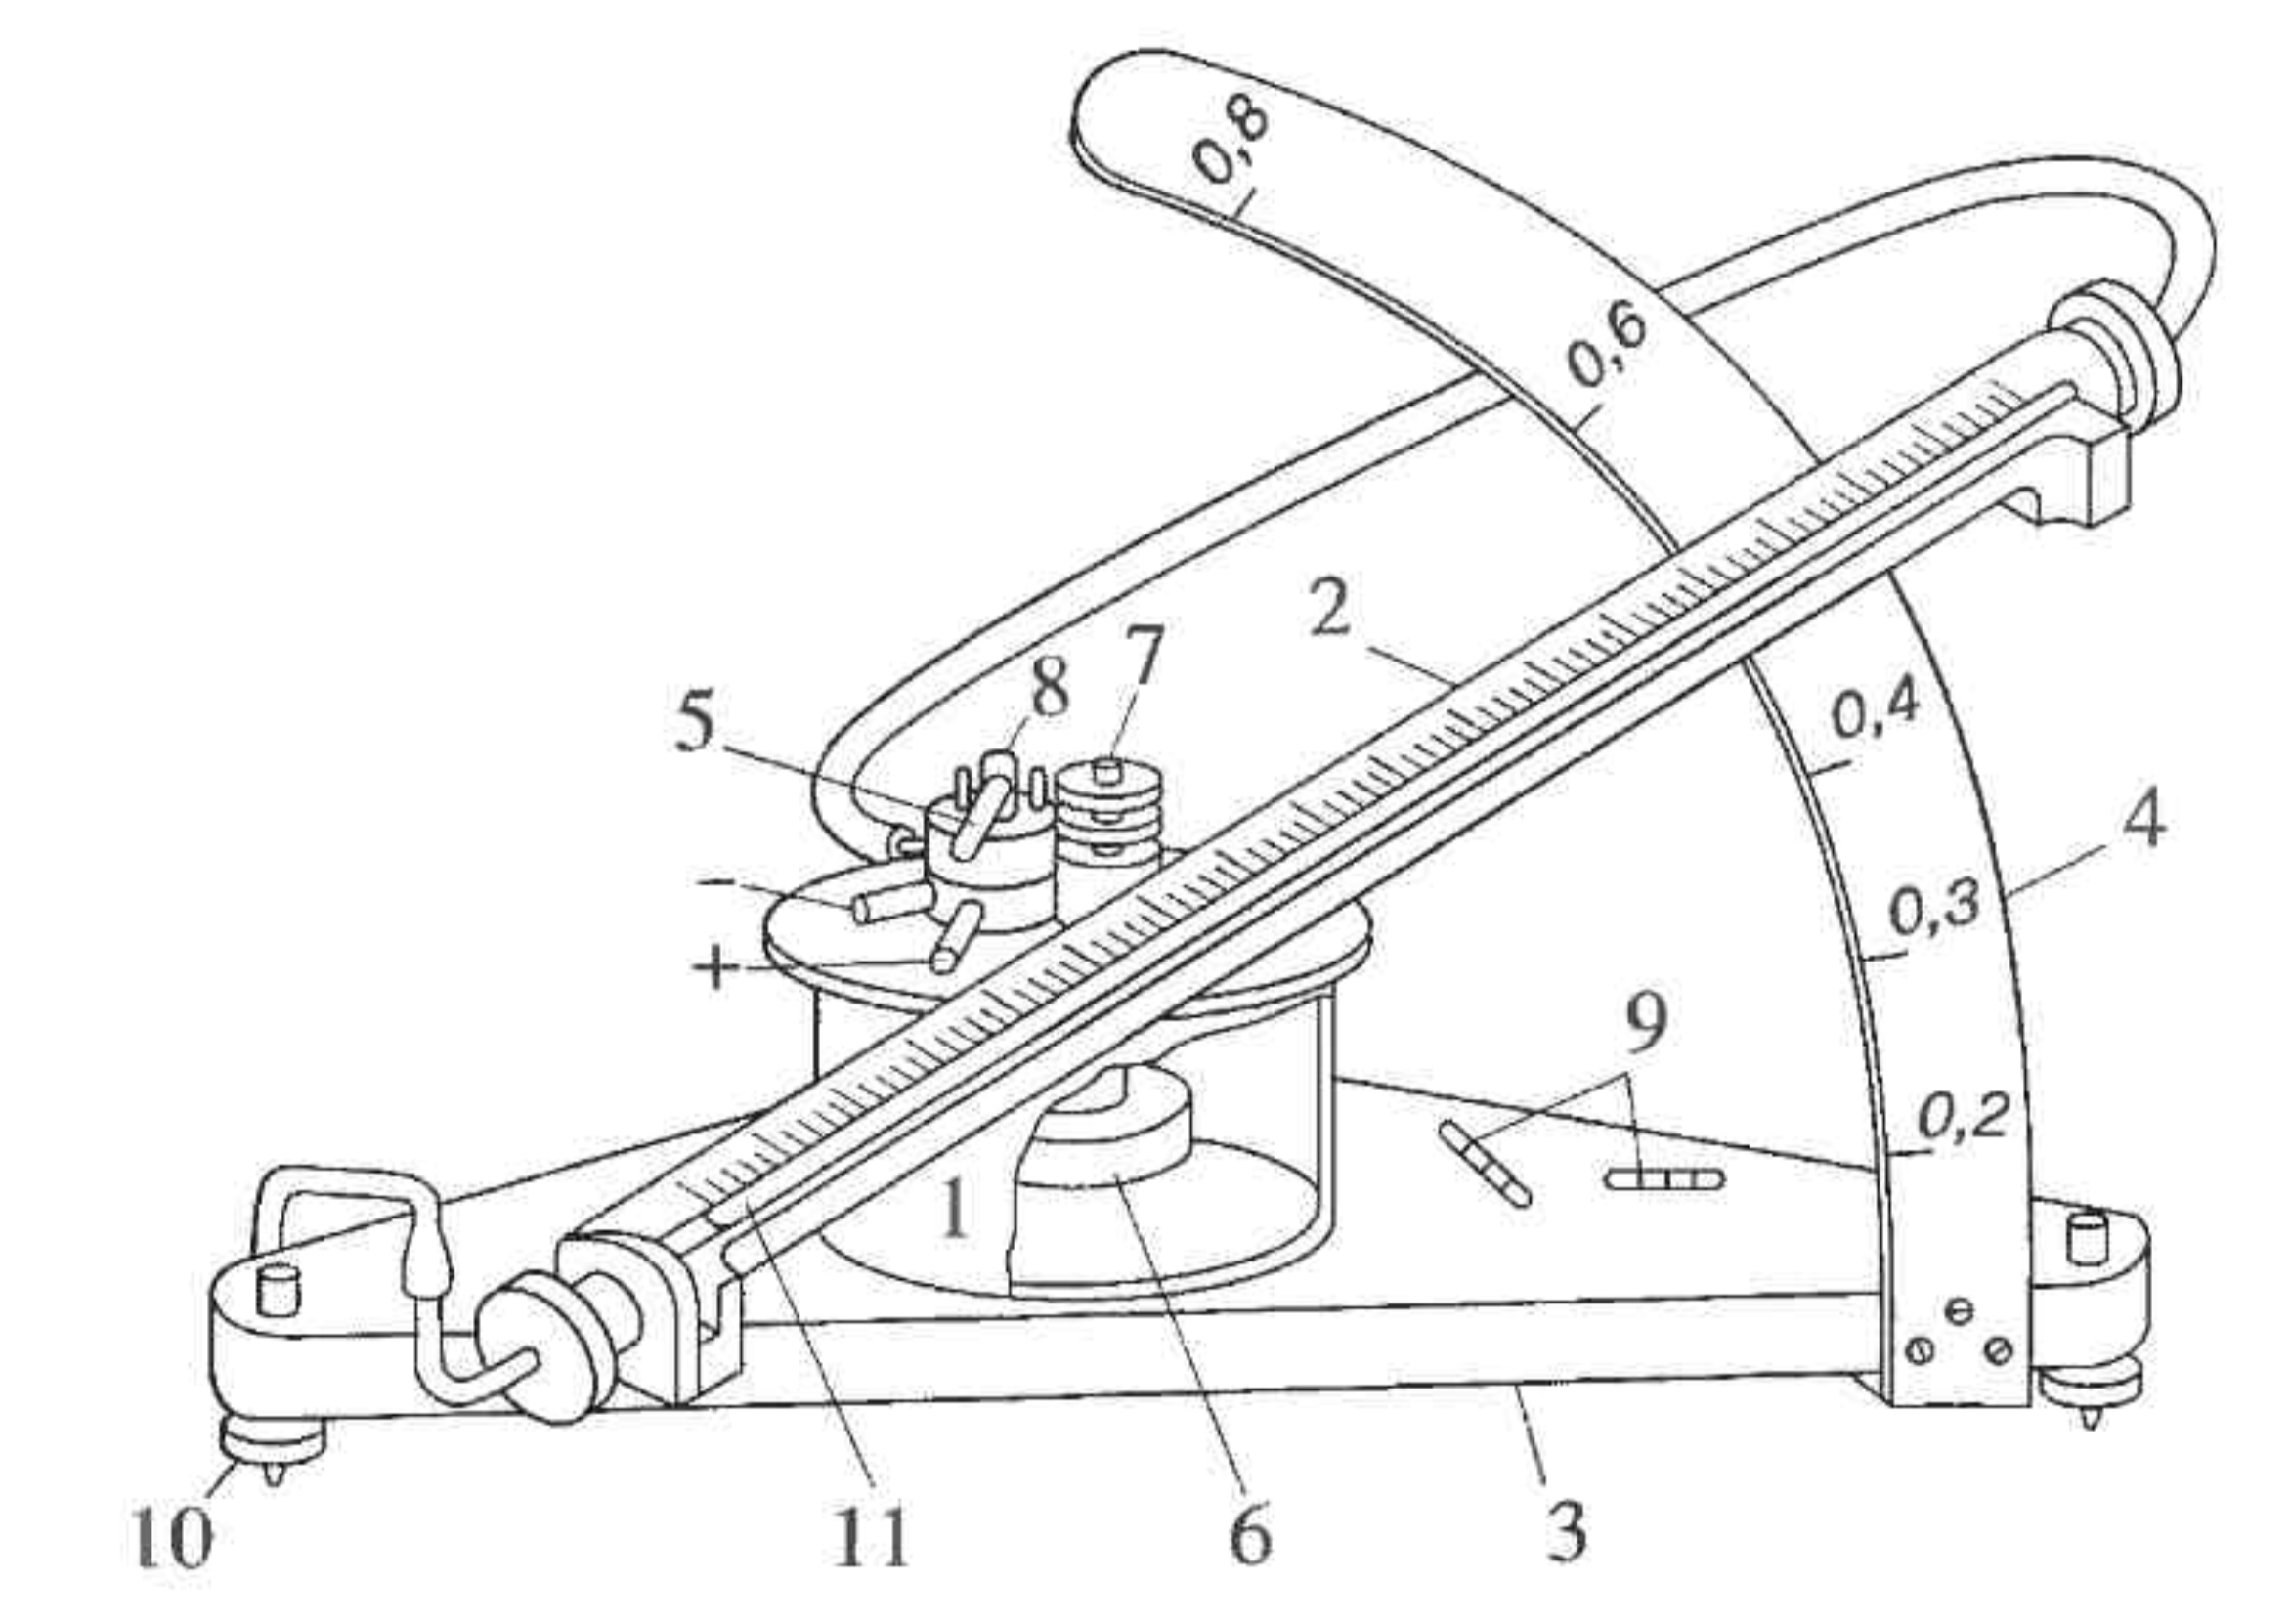
\includegraphics[width=\linewidth]{3}
    \captionsetup{justification=centering}
    \caption{Схема установки для измерений $e/m$ методом магнетрона}
\end{wrapfigure}


Схема установки приведена на Рис.~3. Двухэлектродная лампа Л с цилиндрическим анодом специально
изготовлена из немагнитных материалов. Анод лампы состоит из трёх металлических (нержавеющая сталь)
цилиндров одинакового диаметра.

Два крайних цилиндра электрически изолированы от среднего небольшими зазорами и используются для
устранения краевых эффектов на торцах среднего цилиндра, ток с которого используется при измерениях.
В качестве катода используется тонкая (диаметром 50 мкм) хорошо натянутая вольфрамовая проволока,
расположенная по оси всех трёх цилиндров анодной системы. Катод лампы разогревается переменным
током, отбираемым от стабилизированного источника питания. С этого же источника на анод лампы
подаётся постоянное напряжение $V_\text{а}$
(0-120 В), регулируемое с помощью потенциометра и измеряемое вольтметром $V$.

Лампа закреплена в соленоиде. Магнитное поле в соленоиде создаётся постоянным током (Рис. 3), сила которого регулируется ручками источника питания и измеряется амперметром A

Индукция магнитного поля в соленоиде рассчитывается по току $I_\text{м}$, протекающему через обмотку соленоида. 

\section{Результаты измерений и обработка результатов}
\subsection*{Метод магнитной фокусировки}
Ускоряющее напряжение $V$ :
\[
    V = 0,94 \pm 0,02\ \text{кВ}
\] 

Путь электрона $l$ :
\[
    l = 26,5 \pm 0,1\ \text{см}
\] 

Площадь поперечного сечения, умноженная на число витков $SN$ :
\[
    SN = 3000 \pm 100\ \text{см}^2
\] 

Откалибруем милливеберметр. $\Phi_1$ -- начальное положение стрелки. $\Phi_2$ -- положение стрелки,
после размыкания ключа, когда в системе был ток $I$. Вычислим магнитную индукцию при
фокусировке $B_\text{ф}$ по формуле $B_\text{ф}
= |\Phi_1-\Phi_2|/SN$
\renewcommand{\arraystretch}{1.2} 
% \renewcommand{\tabcolsep}{1cm} 
\begin{table}[H]
\centering
\begin{tabular}{|c|c|c|c|c|}
\hline
\begin{tabular}{c} Направление \\ движения\\ тока \end{tabular}& $\Phi_1, \ \text{мВб}$ &
$\Phi_2,\ \text{мВб}$   & $I,\ \text{А}$ & $B_\text{ф}, \text{мТл}$  \\ \hline
\multirow{5}{*}{В одну сторону} & 4 & 3,2 & 0,59 & 2,67  \\ \cline{2-5} 
                                & 4 & 2,4 & 1,19 & 5,33  \\ \cline{2-5} 
                                & 4 & 1,6 & 1,78 & 8,00  \\ \cline{2-5} 
                                & 5 & 1,7 & 2,4  & 11,00 \\ \cline{2-5} 
                                & 6 & 1,9 & 2,98 & 13,67 \\ \hline
\multirow{5}{*}{В другую}       & 5 & 5,7 & 0,6  & 2,33  \\ \cline{2-5} 
                                & 5 & 6,6 & 1,2  & 5,33  \\ \cline{2-5} 
                                & 5 & 7,3 & 1,77 & 7,67  \\ \cline{2-5} 
                                & 4 & 7,2 & 2,37 & 10,67 \\ \cline{2-5} 
                                & 3 & 6,9 & 2,92 & 13,00 \\ \hline
\end{tabular}
\captionsetup{justification=centering}
\caption{Калиброка миливеберметра}
\end{table}

Снимем зависимость $I_\text{ф}$ от номера фокуса $n$:
\begin{table}[H]
\centering
\begin{tabular}{|c|c|c|c|}
\hline
\multicolumn{2}{|c|}{\begin{tabular}{c}В одну \\ сторону \end{tabular}} & \multicolumn{2}{c|}{В другую} \\ \hline
n           & $I_\text{ф}$   & n            & $I_\text{ф}$  \\ \hline
1           & 0,59           & 1            & 0,6            \\ \hline
2           & 1,2            & 2            & 1,19           \\ \hline
3           & 1,79           & 3            & 1,78           \\ \hline
4           & 2,4            & 4            & 2,36           \\ \hline
5           & 2,99           & 5            & 2,91           \\ \hline
\end{tabular}
\captionsetup{justification=centering}
\caption{Зависимость $I_\text{ф}$ от номера фокуса $n$}
\end{table}

Построим график зависимости $B_\text{ф}$ от тока $I$.
\begin{figure}[H]
    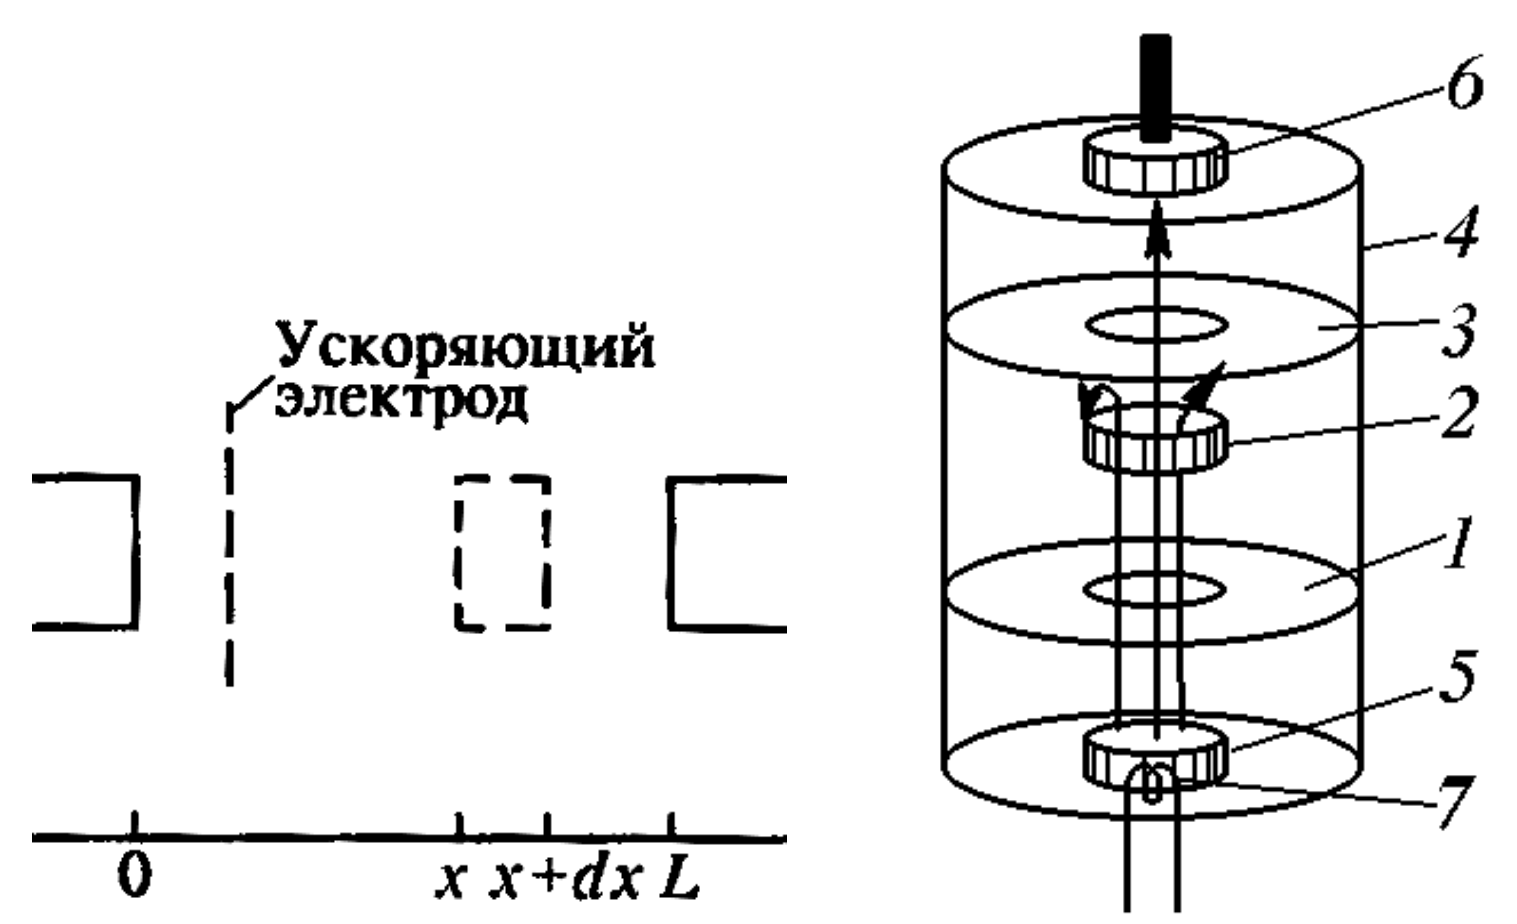
\includegraphics[width=0.9\linewidth]{4}
    \captionsetup{justification=centering}
    \caption{График зависимости $B_\text{ф}$ от тока  $I$}
\end{figure}

Усредняя значение $I_\text{ф}$ и высчитывая значение $B_\text{ф}$ по Рис. 4 построим график
зависимости $B_\text{ф}$ от номера фокуса $n$:

\begin{figure}[H]
    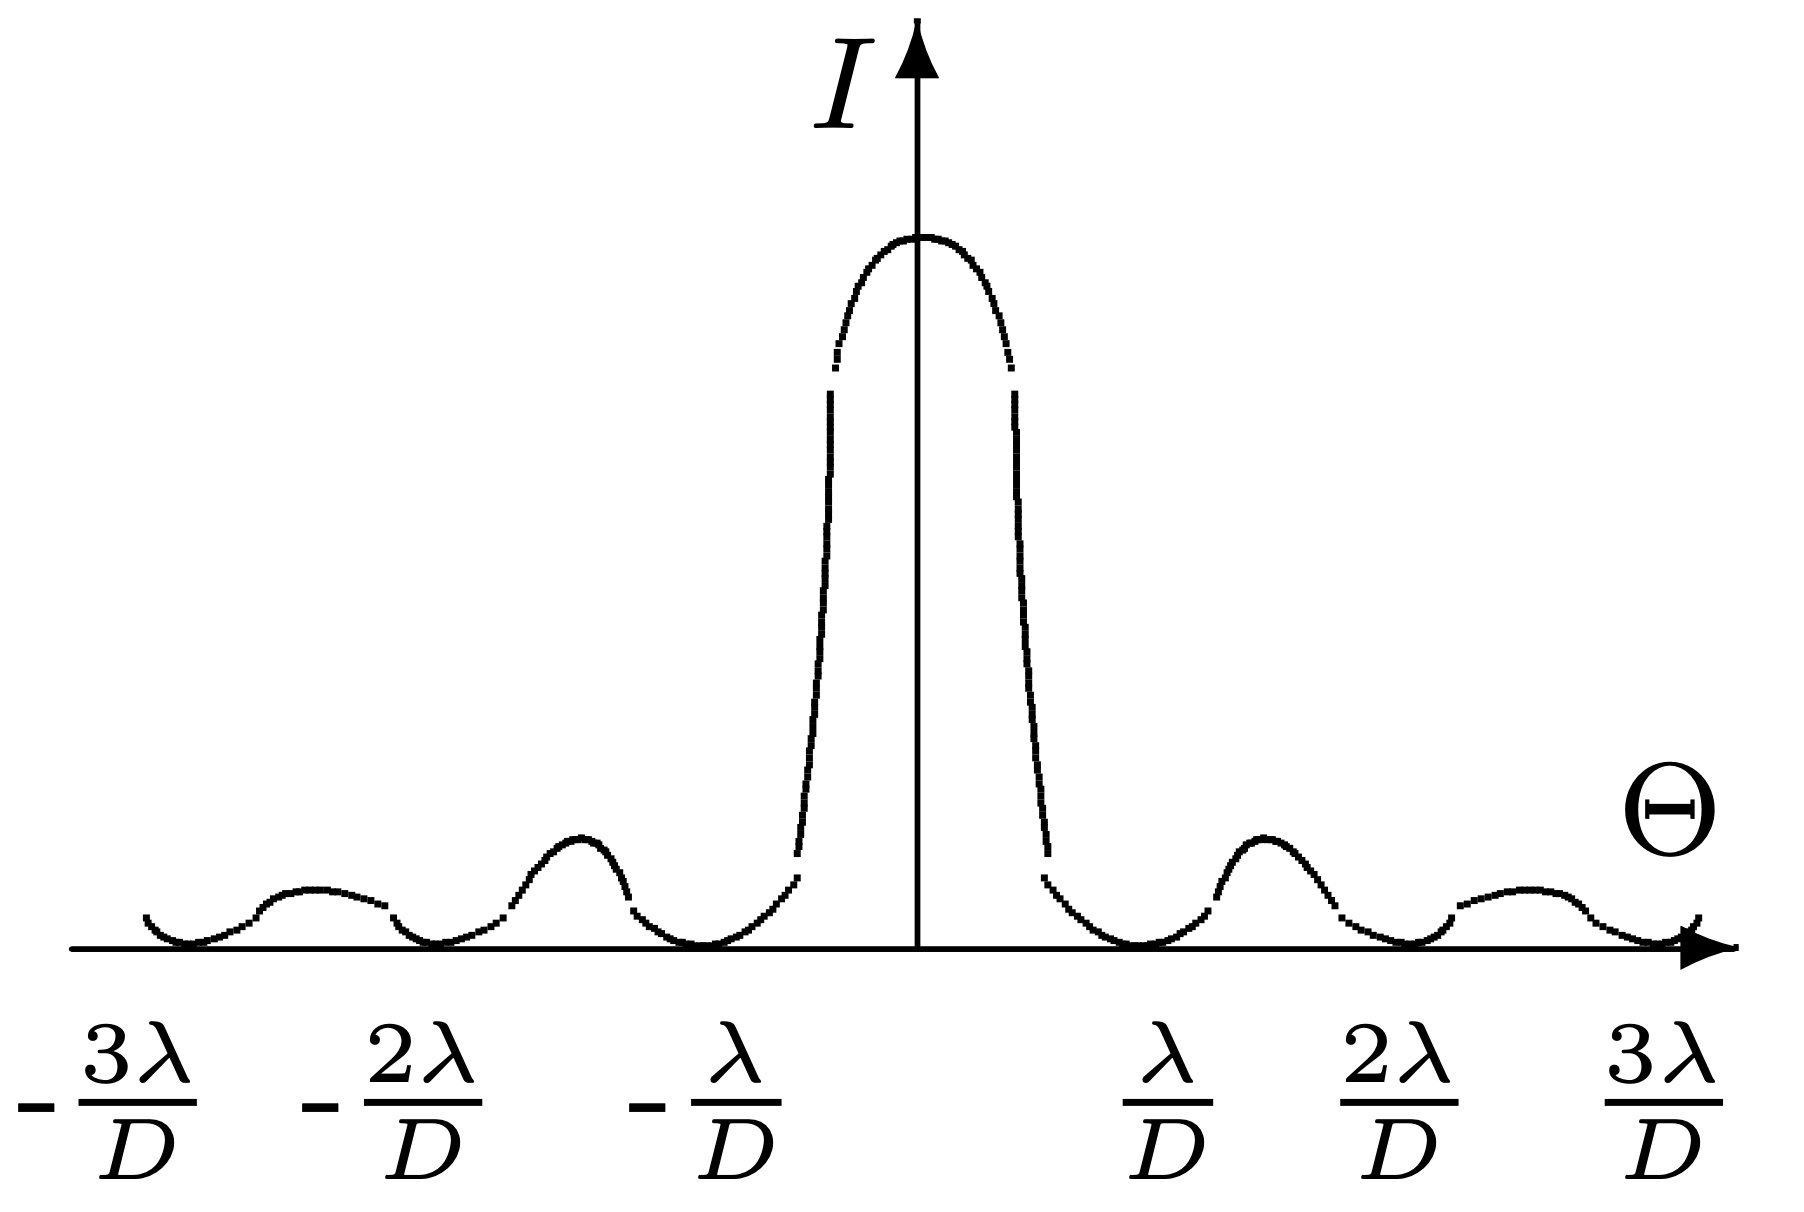
\includegraphics[width=0.9\linewidth]{5}
    \captionsetup{justification=centering}
    \caption{График зависимости $B_\text{ф}$ от номера фокуса $n$}
\end{figure}

По графику на Рис. 5 и по формуле (2) находим удельный заряд электрона.
\[
    \left|\frac{e}{m}\right| = (1,92 \pm 0,05) \cdot 10^{11} \ \text{Кл/кг}
\] 

\subsection*{Метод магнетрона}
Радиус анода:
\[
    r_\text{а} = 12 \pm 1 \ \text{мм}
\] 

Коэффициент пропорциональности между вектором магнитной индукции $B$ и током через соленоид
$I_\text{м}$:
\[
    K = (2,8 \pm 0,1) \cdot 10^{-2} \ \text{Тл/А}
\] 

Снимем зависимость анодного тока $I_\text{а}$ от тока $I_\text{м}$ через соленоид при постоянной
разности потенциалов на аноде лампы $V_\text{а}$. $B$ считаем по формуле $B = KI_\text{м}$
\renewcommand{\arraystretch}{1.15} 
\renewcommand{\tabcolsep}{0.11cm} 

\begin{table}[H]
\centering
\begin{tabular}{|c|c|c||c|c|c||c|c|c||c|c|c|}
\hline
\begin{tabular}{c}$I_\text{а},$\\ $ \text{мкА}$ \end{tabular}      &
\begin{tabular}{c}$I_\text{м},$\\ $ \text{мА}$ \end{tabular}       &
\begin{tabular}{c}$B,$\\ $ \text{мкТл}$ \end{tabular}  &
\begin{tabular}{c}$I_\text{а},$\\ $ \text{мкА}$ \end{tabular}      &
\begin{tabular}{c}$I_\text{м},$\\ $ \text{мА}$ \end{tabular}       &
\begin{tabular}{c}$B,$\\ $ \text{мкТл}$ \end{tabular}  &
\begin{tabular}{c}$I_\text{а},$\\ $ \text{мкА}$ \end{tabular}      &
\begin{tabular}{c}$I_\text{м},$\\ $ \text{мА}$ \end{tabular}       &
\begin{tabular}{c}$B,$\\ $ \text{мкТл}$ \end{tabular}  &
\begin{tabular}{c}$I_\text{а},$\\ $ \text{мкА}$ \end{tabular}      &
\begin{tabular}{c}$I_\text{м},$\\ $ \text{мА}$ \end{tabular}       &
\begin{tabular}{c}$B,$\\ $ \text{мкТл}$ \end{tabular}   \\ \hline
\multicolumn{3}{|c||}{$V_\text{а} = 70\ \text{В}$}    & 
\multicolumn{3}{c||}{$V_\text{а} = 80\ \text{В}$} &
\multicolumn{3}{c||}{$V_\text{а} = 90\ \text{В}$} &
\multicolumn{3}{c|}{$V_\text{а} = 110\ \text{В}$}                \\ \hline
392          & 12           & 336         & 404    & 64    & 1792   & 408     & 108   & 3024   & 412         & 124         & 3472        \\ \hline
416          & 44           & 1232        & 408    & 88    & 2464   & 360     & 136   & 3808   & 380         & 144         & 4032        \\ \hline
400          & 60           & 1680        & 396    & 100   & 2800   & 328     & 152   & 4256   & 344         & 180         & 5040        \\ \hline
384          & 80           & 2240        & 392    & 104   & 2912   & 312     & 160   & 4480   & 320         & 192         & 5376        \\ \hline
376          & 96           & 2688        & 368    & 112   & 3136   & 296     & 172   & 4816   & 280         & 204         & 5712        \\ \hline
344          & 108          & 3024        & 352    & 120   & 3360   & 256     & 184   & 5152   & 256         & 212         & 5936        \\ \hline
332          & 124          & 3472        & 344    & 124   & 3472   & 212     & 188   & 5264   & 180         & 220         & 6160        \\ \hline
300          & 136          & 3808        & 352    & 128   & 3584   & 208     & 192   & 5376   & 104         & 228         & 6384        \\ \hline
276          & 148          & 4144        & 344    & 136   & 3808   & 168     & 196   & 5488   & 48          & 240         & 6720        \\ \hline
252          & 156          & 4368        & 332    & 140   & 3920   & 120     & 200   & 5600   & 24          & 252         & 7056        \\ \hline
236          & 160          & 4480        & 316    & 144   & 4032   & 48      & 208   & 5824   & \multicolumn{3}{c}{\multirow{15}{*}{}} \\ \cline{1-9}
212          & 164          & 4592        & 304    & 148   & 4144   & 24      & 220   & 6160   & \multicolumn{3}{c}{}                   \\ \cline{1-9}
168          & 168          & 4704        & 300    & 152   & 4256   &
\multicolumn{3}{c||}{$V_\text{а} = 100 \ \text{В}$} & \multicolumn{3}{c}{}                   \\ \cline{1-9}
124          & 172          & 4816        & 292    & 156   & 4368   & 420     & 96    & 2688   & \multicolumn{3}{c}{}                   \\ \cline{1-9}
96           & 176          & 4928        & 284    & 160   & 4480   & 408     & 116   & 3248   & \multicolumn{3}{c}{}                   \\ \cline{1-9}
56           & 184          & 5152        & 272    & 164   & 4592   & 368     & 140   & 3920   & \multicolumn{3}{c}{}                   \\ \cline{1-9}
24           & 192          & 5376        & 260    & 168   & 4704   & 344     & 160   & 4480   & \multicolumn{3}{c}{}                   \\ \cline{1-9}
20           & 200          & 5600        & 240    & 172   & 4816   & 300     & 180   & 5040   & \multicolumn{3}{c}{}                   \\ \cline{1-9}
12           & 216          & 6048        & 216    & 176   & 4928   & 280     & 188   & 5264   & \multicolumn{3}{c}{}                   \\ \cline{1-9}
\multicolumn{3}{|c||}{\multirow{2}{*}{$V_\text{а} = 80\ \text{В}$}} & 152    & 184   & 5152   & 256     & 196   & 5488   & \multicolumn{3}{c}{}                   \\ \cline{4-9}
\multicolumn{3}{|c||}{}                    & 180    & 180   & 5040   & 224     & 200   & 5600   & \multicolumn{3}{c}{}                   \\ \cline{1-9}
404          & 12           & 336         & 112    & 188   & 5264   & 164     & 208   & 5824   & \multicolumn{3}{c}{}                   \\ \cline{1-9}
404          & 24           & 672         & 40     & 196   & 5488   & 100     & 216   & 6048   & \multicolumn{3}{c}{}                   \\ \cline{1-9}
404          & 32           & 896         & 24     & 208   & 5824   & 72      & 220   & 6160   & \multicolumn{3}{c}{}                   \\ \cline{1-9}
408          & 40           & 1120        & 4      & 240   & 6720   & 28      & 236   & 6608   &
\multicolumn{3}{c}{}                   \\ \cline{1-9}
\end{tabular}
\captionsetup{justification=centering}
\caption{Зависимость анодного тока $I_\text{а}$ от тока $I_\text{м}$ через соленоид при постоянной
разности потенциалов на аноде лампы $V_\text{а}$}
\end{table}

Погрешность измерения анодного тока $I_\text{а}$ и тока $I_\text{м}$ через соленоид примем равной
цене деления измеряющего эти величины прибора:
\begin{equation*}
    \begin{aligned}
        \Delta I_\text{а} = 4 \ \text{мкА}\\
        \Delta I_\text{м} = 4 \ \text{мА}
    \end{aligned}
\end{equation*}

По результатам в Таблице 3 построим график зависимости  $I_\text{a}$ от $B$. $B_\text{кр}$
определим, усредняя значения $B$ при максимальных перепадах $I_\text{а}$ при малых изменениях $B$.
\begin{figure}[H]
    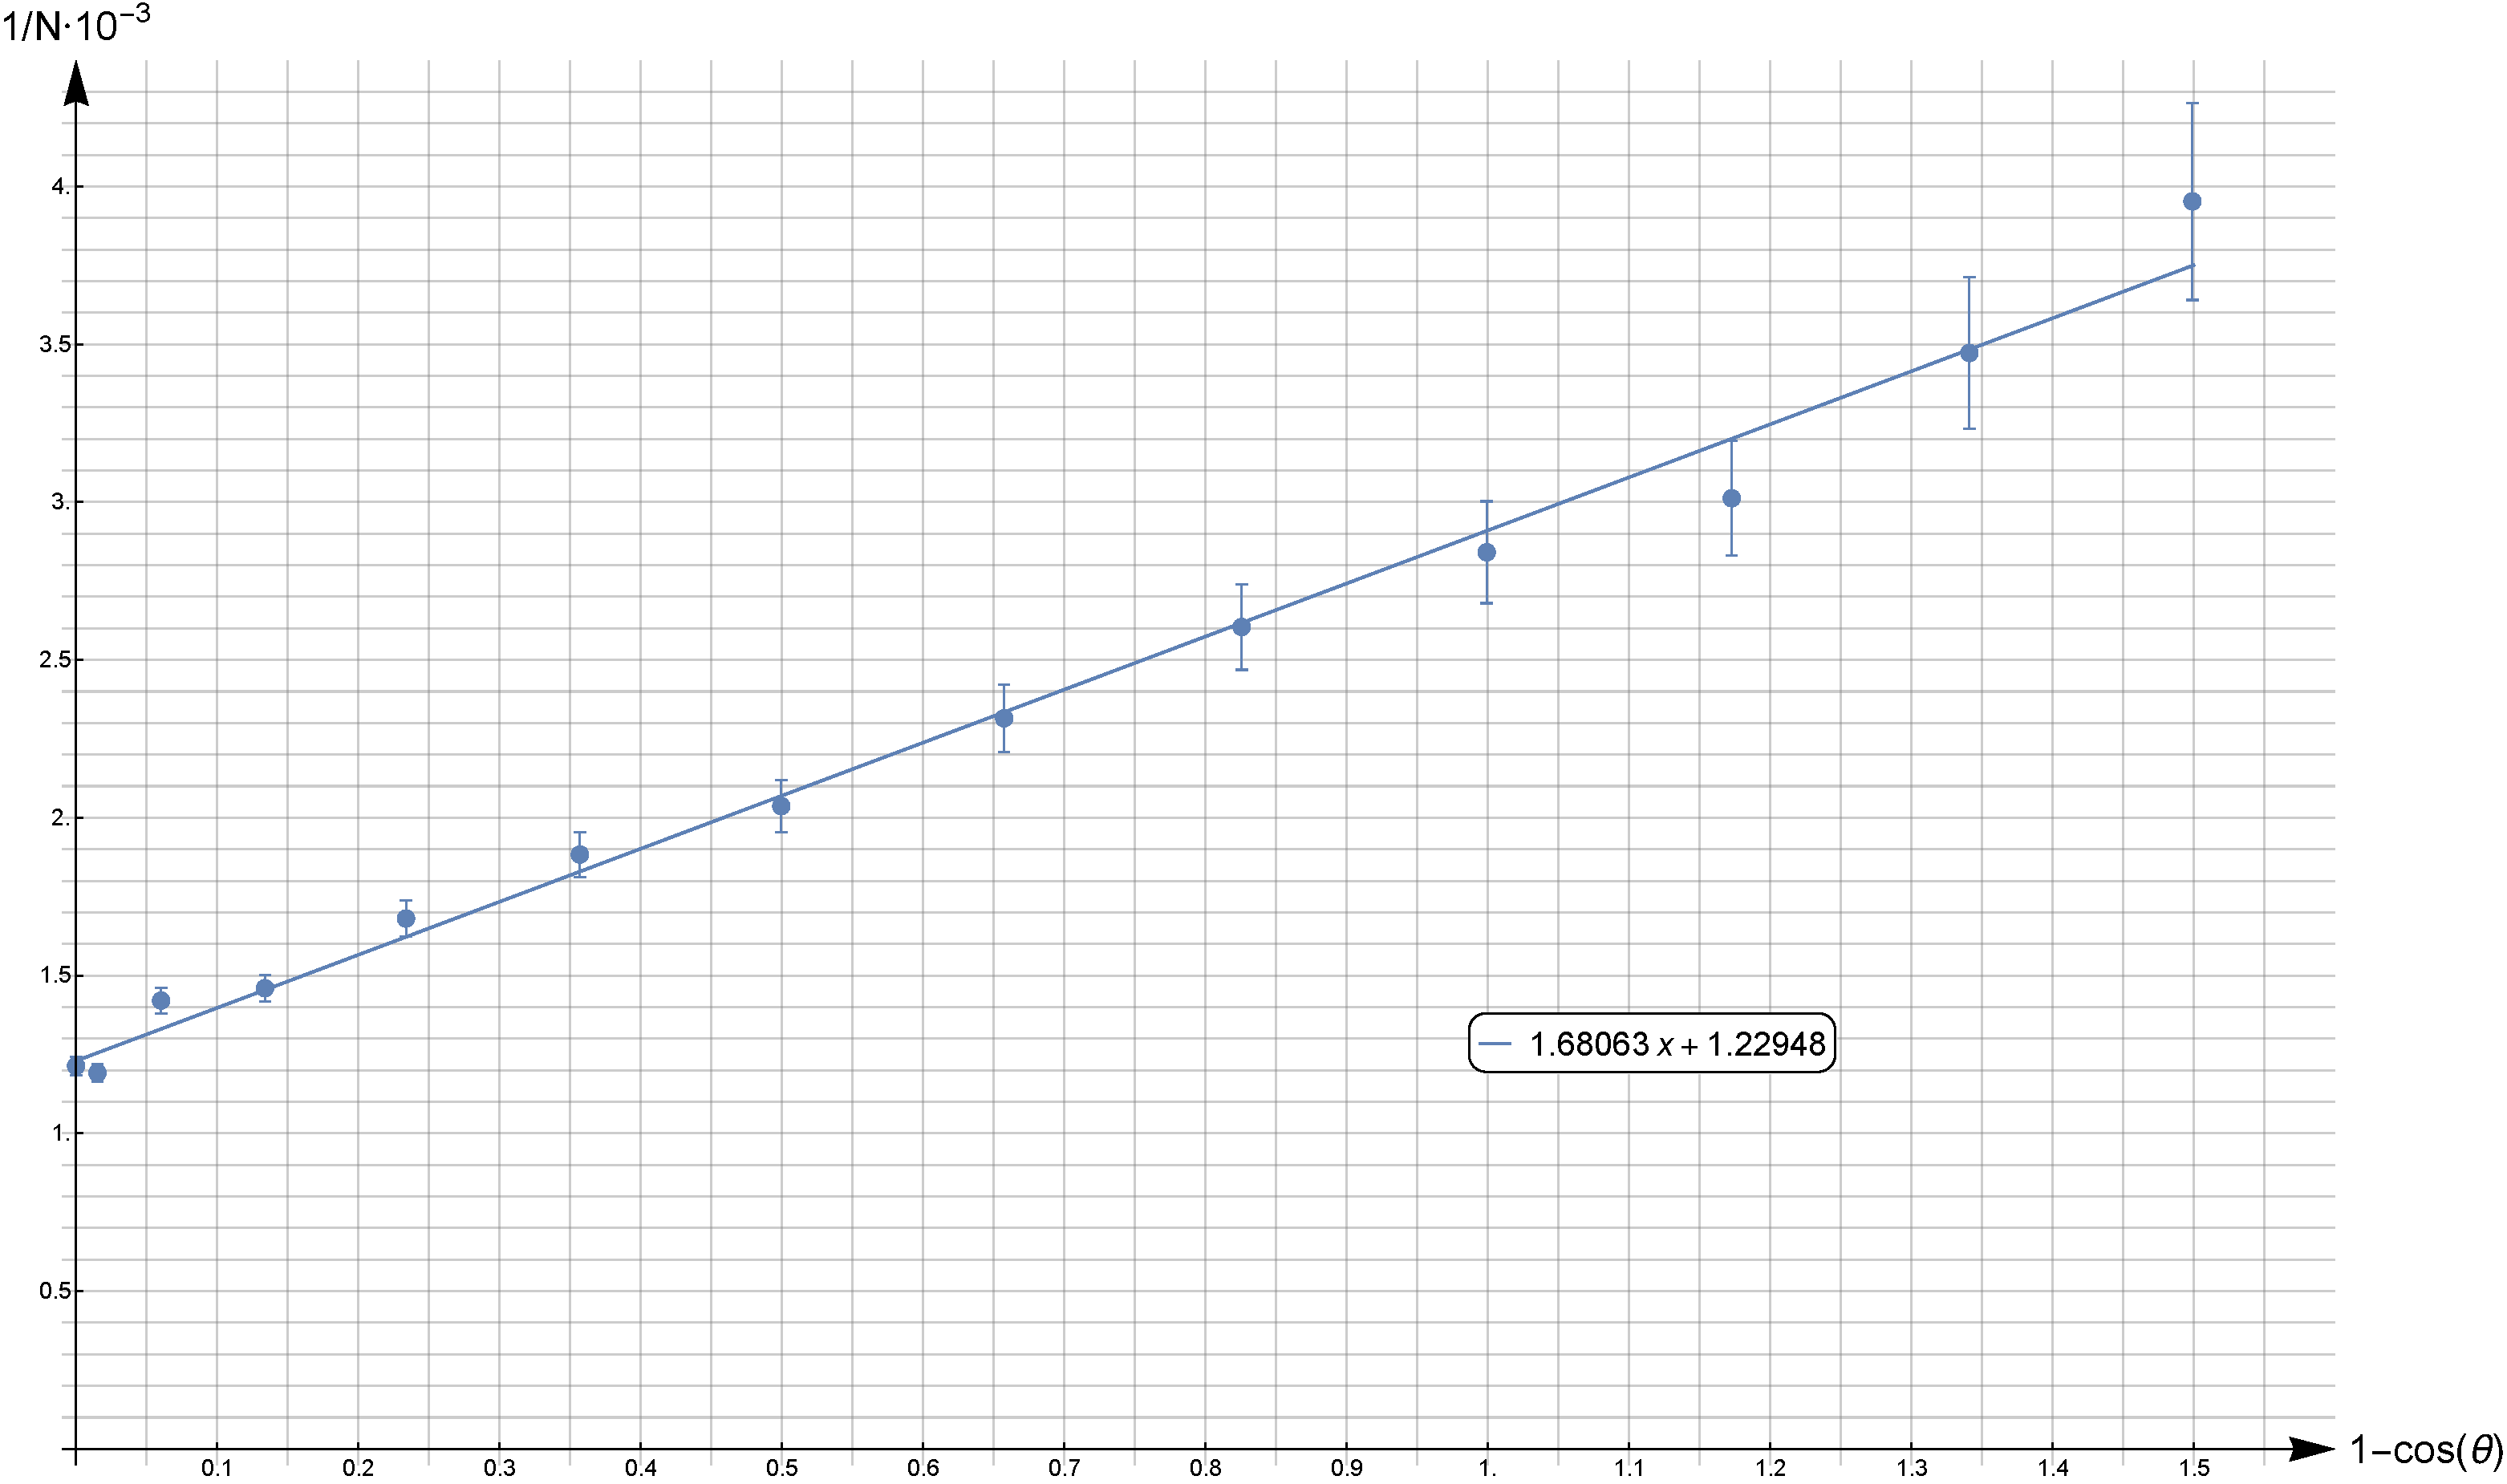
\includegraphics[width=\linewidth]{6}
    \captionsetup{justification=centering}
    \caption{График зависимости $I_\text{а}$ от индукции магнитного поля в соленоиде $B$}
\end{figure}

По графику на Рис. 6 составим таблицу зависимости $B_\text{кр}^2$ от $V_\text{а}$
\begin{table}[H]
\centering
\begin{tabular}{|c|c|c|c|}
\hline
$B_\text{кр}^2,\ \text{Тл} \cdot 10^{-6}$        & $\Delta B_\text{кр}^2,\ \text{Тл} \cdot 10^{-6}$
& $V_\text{а}, \ \text{В}$   & $\Delta V_\text{а}, \ \text{В}$  \\ \hline
22,37   & 2,37 & 70  & 1,4 \\ \hline
24,98 & 2,50 & 80  & 1,6 \\ \hline
28,73   & 2,68  & 90  & 1,8 \\ \hline
31,72 & 2,82 & 100 & 2,0   \\ \hline
34,81     & 2,95  & 110 & 2,2 \\ \hline
\end{tabular}
\captionsetup{justification=centering}
\caption{Зависимость квадрата критического значения магнитной индукции магнитного поля в соленоиде  $B_\text{кр}$ от
потенциала на аноде лампы $V_\text{a}$}
\end{table}

По результата в Таблице 4 построим график зависимости квадрата критического значения магнитной
индукции $B_\text{кр}$ от потенциала на аноде лампы $V_\text{а}$

\begin{figure}[H]
    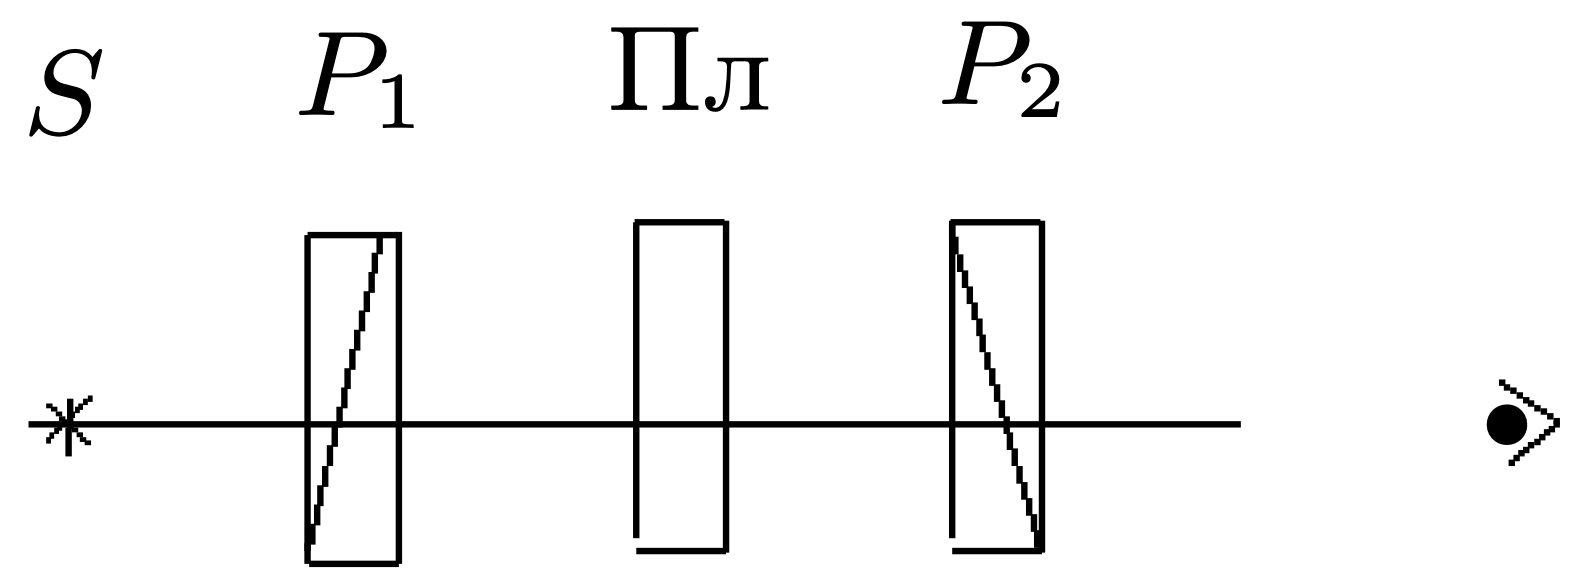
\includegraphics[width=\linewidth]{7}
    \captionsetup{justification=centering}
    \caption{График зависимости квадрата критического значения магнитной
индукции $B_\text{кр}$ от потенциала на аноде лампы $V_\text{а}$
}
\end{figure}
 
Использую формулу (3) вычислим удельный заряд электрона:
\[
    \left| \frac{e}{m}\right| = (1,8 \pm 0,2) \cdot 10^{11}\ \text{Кл/кг}
\] 
\section{Обсуждение результатов и выводы}
В работе был определен удельный заряд электрона методом магнитной фокусировки и методом
магнетрона.

\textbf{Метод магнитной фокусировки:}
\[
    \left|\frac{e}{m} \right| = (1,92\pm 0,05) \cdot 10^{11}\ \text{Кл/кг} 
\] 

\textbf{Метод магнетрона:}
\[
    \left|\frac{e}{m} \right| = (1,8\pm 0,2) \cdot 10^{11}\ \text{Кл/кг}
\] 

Результат, полученный методом магнитной фокусировки, получился несколько завышен. Это может быть связано с
влиянием магнитов, находящихся не далеко от установки, на показания миливеберметра.

\end{document}
